\section{System Architecture} \label{sec:sysarc}


The control system architecture is a relatively flat DDS message based system using multi cast messaging. A high level view is given in \figref{fig:arc}



\begin{figure}
\begin{center}
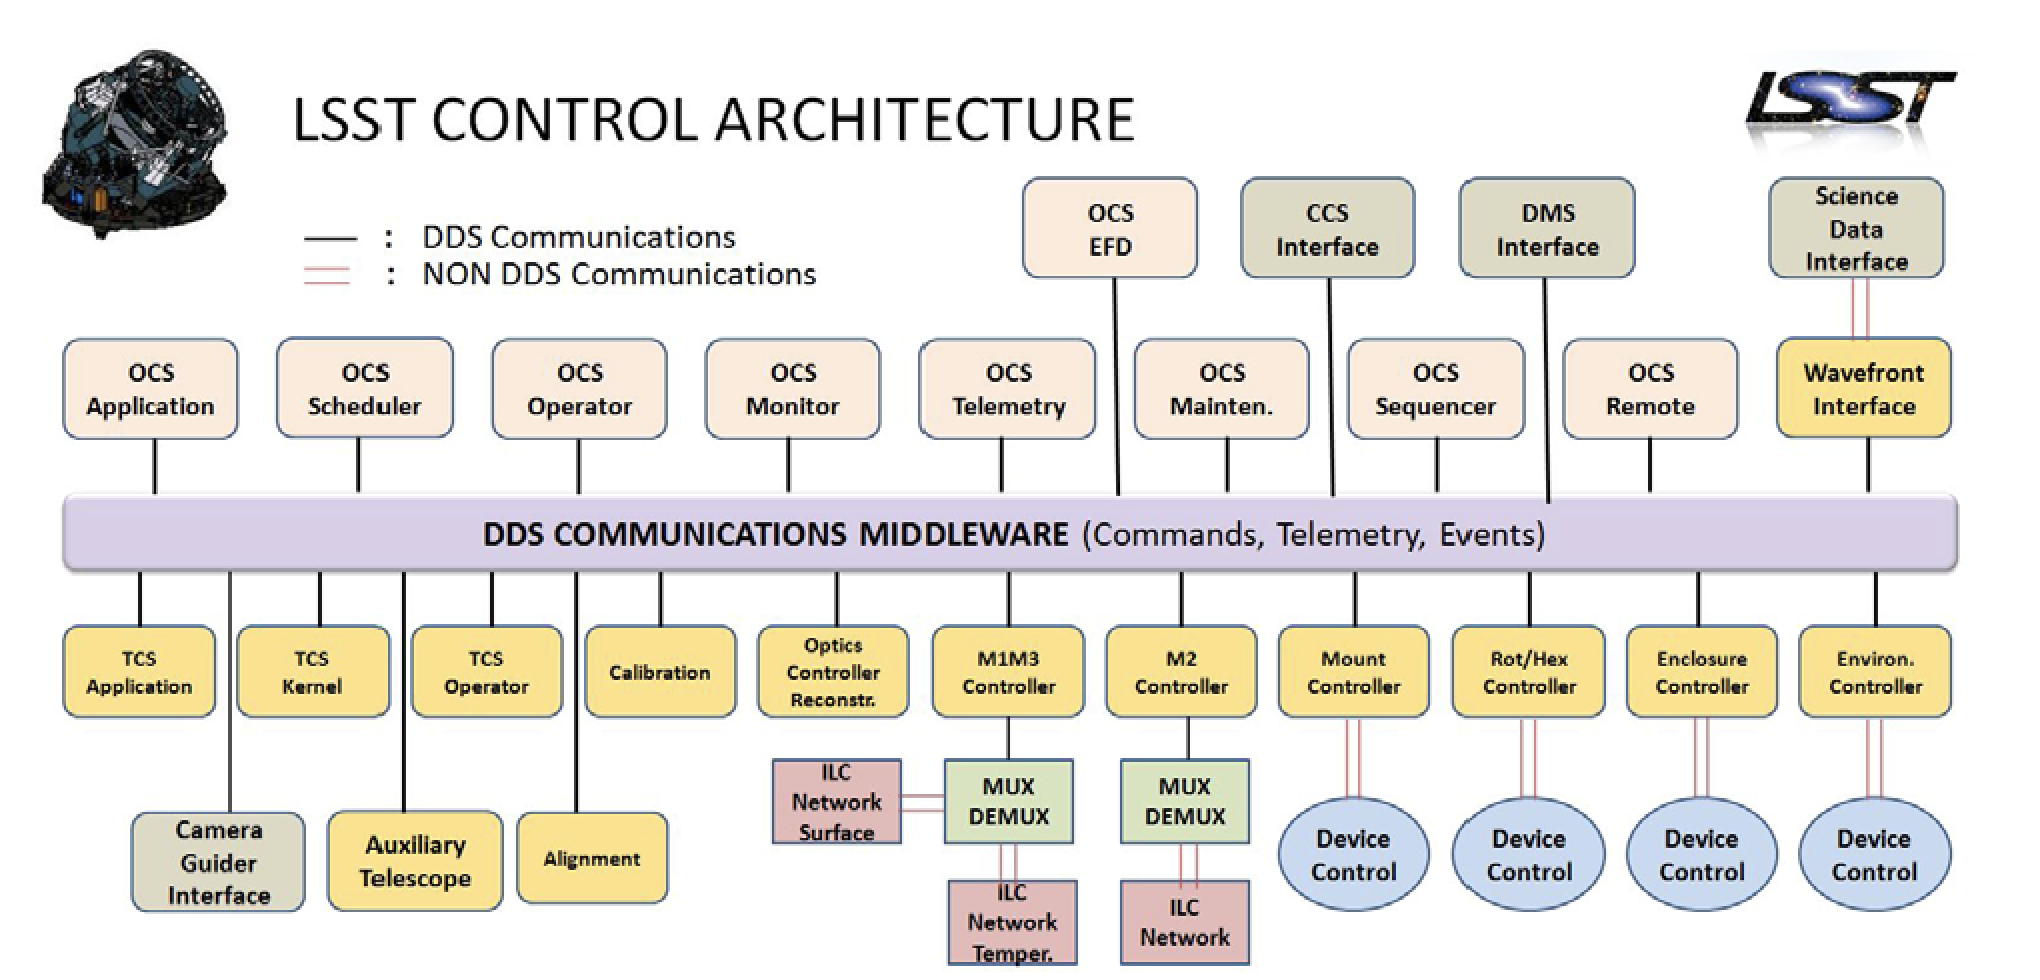
\includegraphics[width=0.8\textwidth]{arc}
\caption{High Level Architecture Diagram\label{fig:arc}}
\end{center}
\end{figure}

Broadly this may be seen as comprising:
\begin{itemize}
\item Infrastructure and Middleware :
	\begin{itemize}
	\item Service Access Layer (SAL) based on DDS
	\item Engineering and Facility Database (EFD)
	\item Operator Interface (based on LOVE)
	\item Script Queue  \footnote{\url{https://github.com/lsst-ts/ts_scriptqueue}}
	\item Python Scripting based on SalObj\footnote{\url{https://github.com/lsst-ts/ts_salobj}}
	\end{itemize}
\item The Scheduler \footnote{\url{https://github.com/lsst-ts/ts_scheduler}}
\item Potentially an Auxiliary and Main Telescope Control System (ATCS and TCS)\footnote {The precise nature and need for these is unclear now so they have lower priority.}
\item Controllable SAL Components (CSCs) - every device and some pseudo devices, including the scheduler, are CSCs. Some are coordinating other CSCs, the full hierarchy is shown for AuxTel in \figref{fig:atcscs} and the Main Telescope in \figref{fig:mtcscs}
\end{itemize}

\begin{figure}
\begin{center}
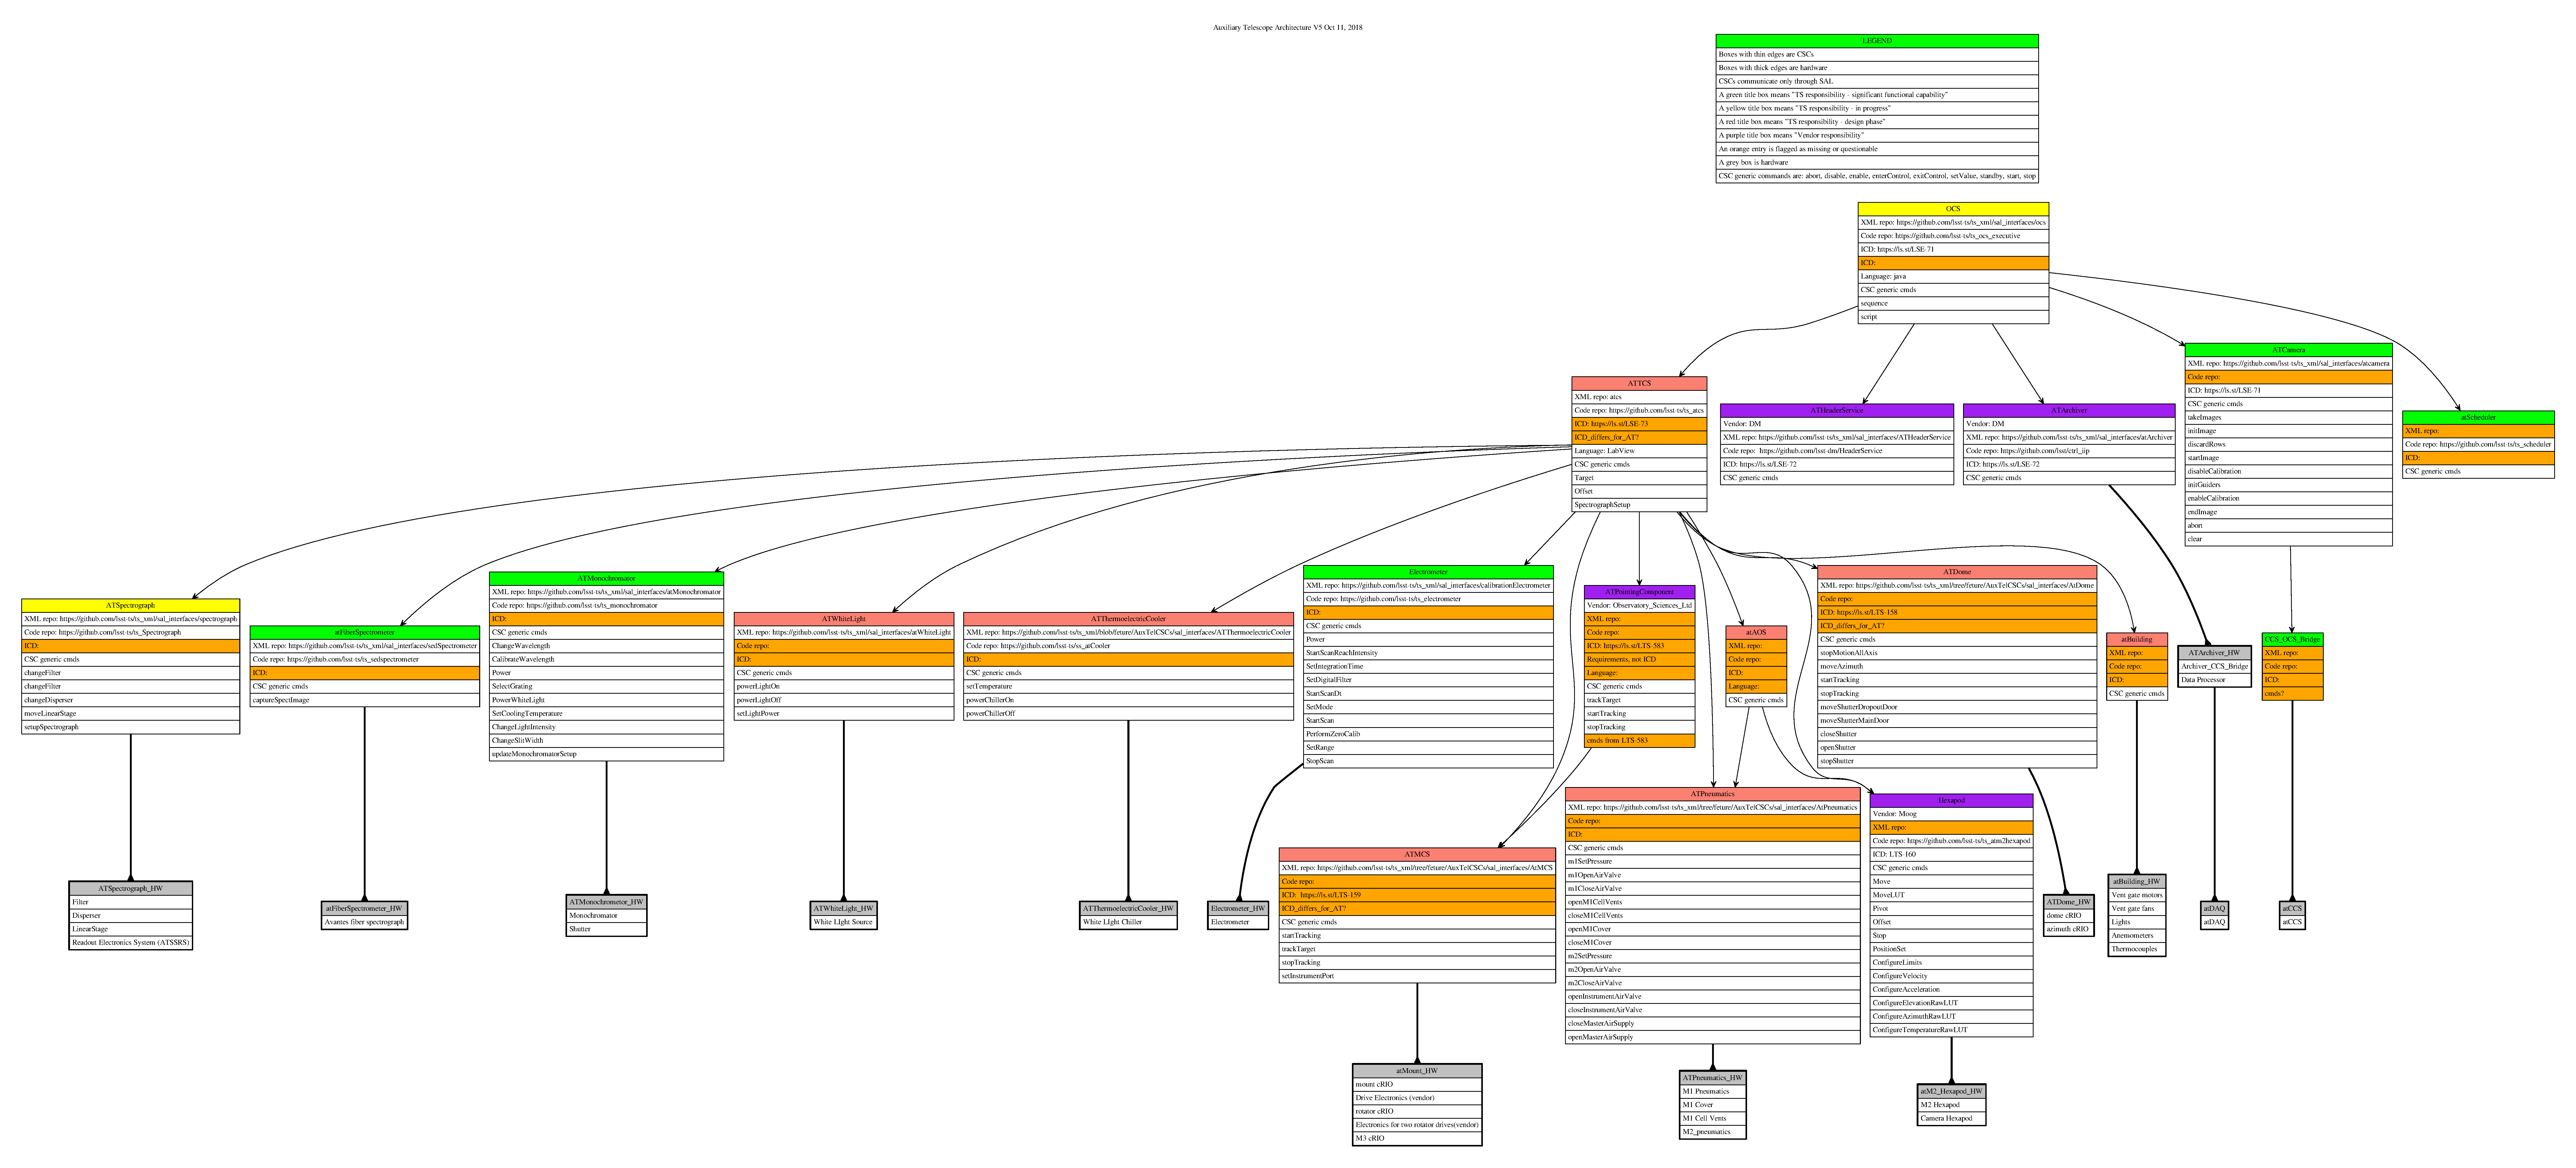
\includegraphics[width=0.9\textwidth]{AT}
\caption{Complete set of AuxTel CSCs\label{fig:atcscs}}
\end{center}
\end{figure}

\begin{figure}
\begin{center}
\includegraphics[width=0.9\textwidth]{LSST}
\caption{Complete set of Main Telescope CSCs\label{fig:mtcscs}}
\end{center}
\end{figure}

\subsection{SalObj - Python and scripting }\label{sect:salobj}
The SalObj Python library provides a handy way of creating Controllable SAL Components (CSCs) which are not time critical. It also provides the basis for attaching to and scripting any orchestration of CSCs. A high level diagram is provided in \figref{fig:salobj}.

\begin{figure}
\begin{center}
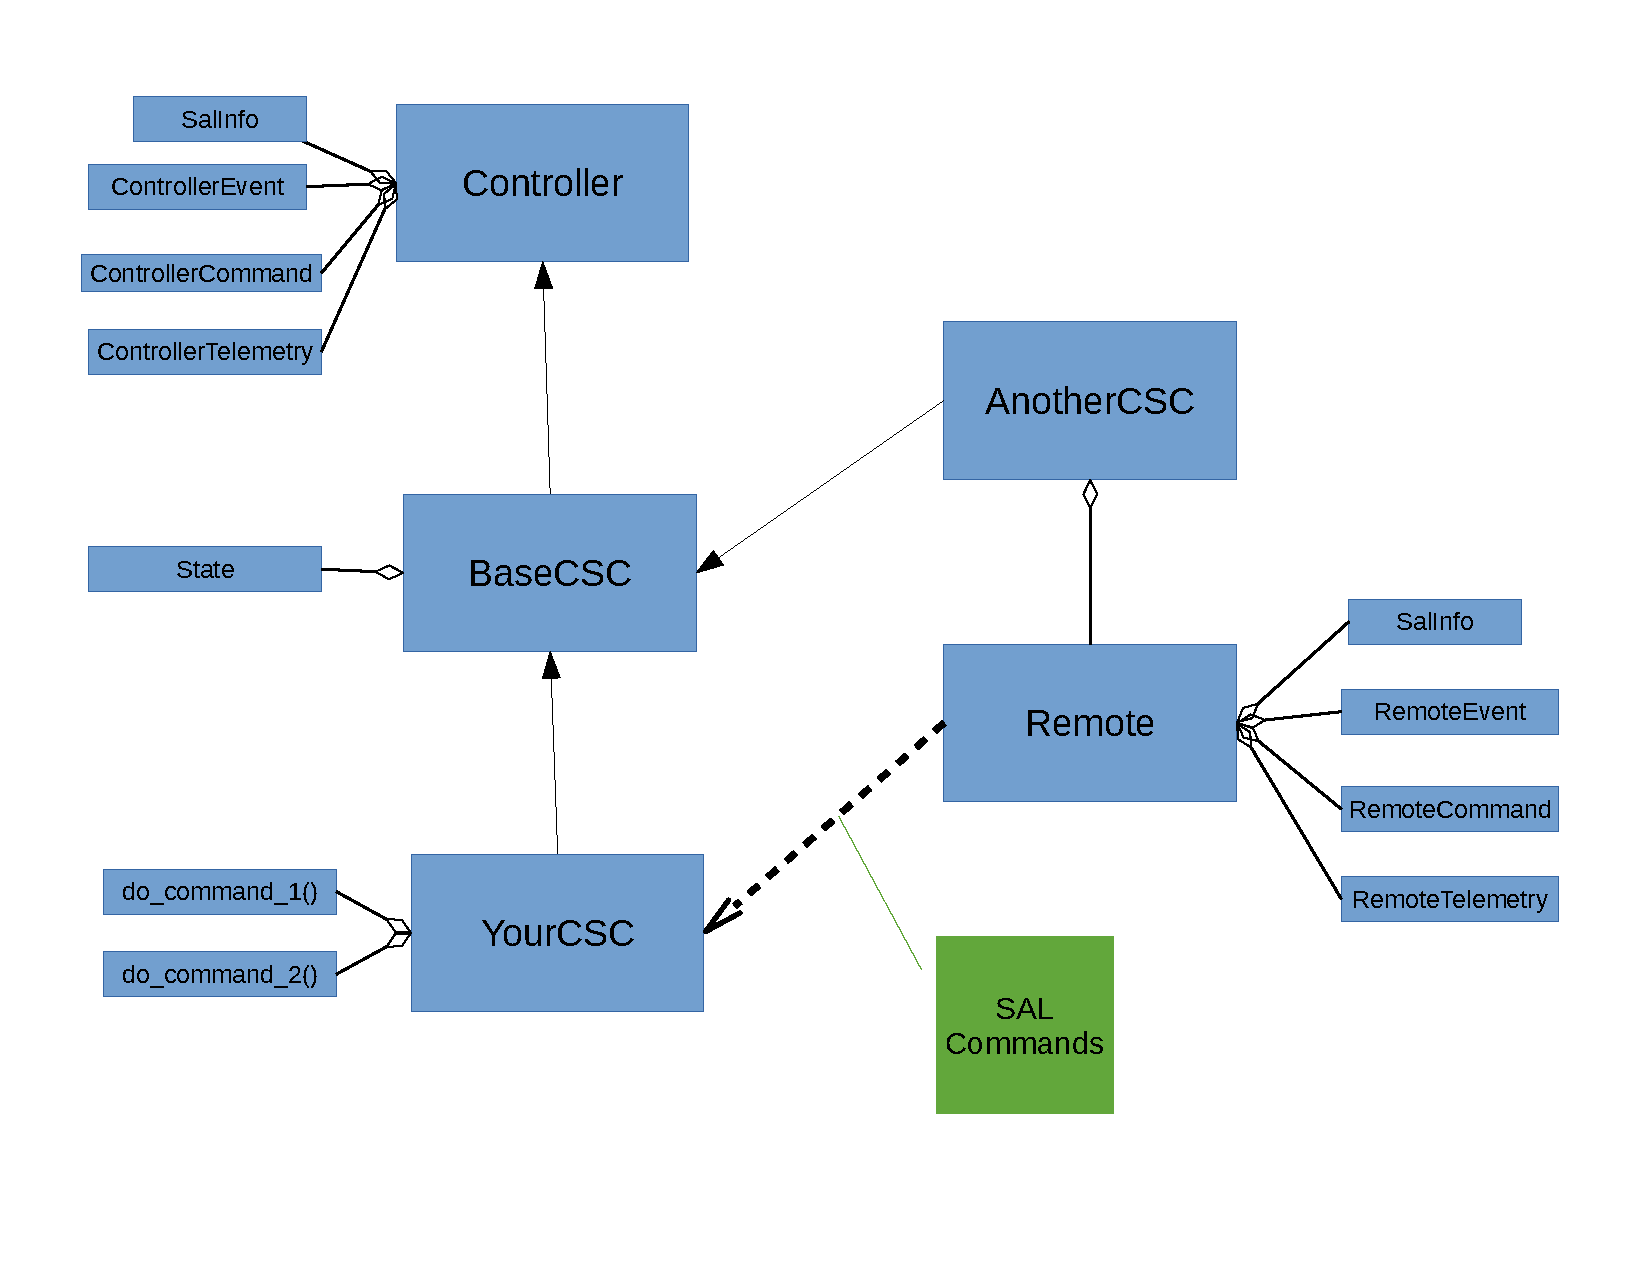
\includegraphics[width=0.9\textwidth]{SalobjClassDiag2}
\caption{SalObj python scheme for  CSCs\label{fig:salobj}}
\end{center}
\end{figure}

\subsection{ScriptQueue} \label{sect:scriptq}
The LSST control system is run by the ScriptQueue, the contents of which are Python Scripts.
As Python programs, these scripts have access to all Python functionality, both from the native
Python 3 language and through imported modules, including asyncio to manage parallel
activities. In particular, a Script has access to all system components through the salobj (\secref{sect:salobj})
module, which implements SAL communication with CSCs (Commandable SAL Components).
In such an environment it is not immediately clear that a traditional hierarchical design is
necessary or desirable. A completely flat architecture initially seems completely workable and certainly sufficient during in AIT and early commissioning.
For example, consider a Script which commands and sequences the telescope subsystems to move
to the next field to be observed, take an exposure, and read out that exposure. The Script can
directly control each of those subsystems and maintain control of the sequencing using asyncio.
Furthermore, the complexity of the Script can be managed through normal modular
programming techniques, in which subsystem functionality is implemented through Python
objects imported in modules.

\subsection{Observatory Control System } \label{sect:ocs}
Though we could have a flat system based on ScriptQueue (\secref{sect:scriptq})
there are two compelling reason to retain at least a top level OCS which has
overall responsibility for all subsystems. The first reason is rooted in the limited lifetime of each
Script, which has an execution thread that begins and ends over a duration short compared to
the up time of the telescope system. When a Script is instantiated, it has no immediate
knowledge of the state of the telescope system as a whole, or the state of individual
subsystems. It needs such knowledge, because many actions, e.g. moving the telescope,
require the telescope subsystems to be in particular states. The Script can of course assemble
the required knowledge, by using SAL to obtain the state information of all relevant subsystems,
but doing so imposes unnecessary startup overheads for Scripts. It is far more efficient, not to
say reliable, for a single subsystem to be continuously responsible for maintaining knowledge of
the overall state of the observatory (observatory states are discussed in more detail below)

The second, related, reason is that the operator needs:
\begin{enumerate}
\item to maintain continuous knowledge of
the state of the observatory independent of Script execution, and
\item  to be able to command the
observatory to change its overall state.
\end{enumerate}
An excellent example of the latter requirement is from
the LOVE requirements document, \citeds{LTS-807}: “The LOVE shall provide a single control
command labeled “Emergency Close” of the telescopes”. Certainly one could imagine creating
a Script to execute “Emergency Close”, but to use it would require that any currently running
Script be aborted, and the “.

It should be noted this could also be achieved by an "Emergency Close" script inserted on top of the ScriptQueue and an abort on the current running script (if there is one) - the ScriptQueue supports this.  So the OCS remains a low priority to be developed during commissioning as we understand the needs better.
